\documentclass[8pt]{beamer}
\usepackage[T1]{fontenc} 
\usepackage[francais]{babel}
\usepackage{tikz}
\usetikzlibrary{arrows,shapes}
\usepackage{pslatex}
\usepackage{textcomp}
\usepackage[utf8]{inputenc}  
\usepackage{wrapfig}
\usepackage{graphicx}
\usepackage[section]{placeins}
\usepackage{lscape}
\usepackage{float} 
\usepackage{amssymb}
\usepackage{wasysym}
\usepackage{pgf}
\usepackage{alltt}
\usepackage{eso-pic}
\usepackage{url}
\usepackage{tikz}
\usepackage{listings}
\usepackage{color}
\definecolor{mymauve}{rgb}{0.58,0,0.82}

\lstset{language=C++,
basicstyle=\footnotesize,
keywordstyle=\color{red}\bfseries,
breaklines=true,
commentstyle=\color{blue},
stringstyle=\color{mymauve},
literate={ô}{{\^o}}1 {é}{{\'e}}1 {à}{{\`a}}1 {è}{{\`e}}1 {î}{{\^{\i}}}1 {ê}{{\^e}}1 {ç}{{\c c}}1,
morekeywords={string,fstream,ofstream,ifstream}
}
\usepackage{hyperref}

%\hypersetup{urlcolor=blue}

\usetheme{CambridgeUS}


\title[DQM4HEP]{Data Quality Monitoring for High Energy Physics (DQM4HEP) \\ Version 03-02-00}
\institute[UCBL - IPNL - UGent]{Université Claude Bernard Lyon 1 - Institut de Physique Nucléaire de Lyon / Ghent University}
\author[Eté - Pingault - Mirabito]{{\bf \large Eté Rémi, Antoine Pingault, Laurent Mirabito}}
\date{\today}

\DeclareUnicodeCharacter{00A0}{ }

\setbeamertemplate{itemize items}[ball]
\definecolor{MyGreen}{rgb}{0.1,0.5,0.1}
\setbeamercolor{structure}{fg=red!70!black}
\setbeamercolor{block title}{bg=red!70!black,fg=black}
\addtobeamertemplate{block begin}{\pgfsetfillopacity{0.5}}{\pgfsetfillopacity{1}}

\begin{document}


  %%%%%%%%%%%%%% Page de présentation %%%%%%%%%%%%%%
  \begin{frame}

    \titlepage
    \begin{center} 
      
\includegraphics[width=0.5\textwidth]{logo/logo-ucbl-ipnl.jpg} ~~~~~~~~~~~
      
\includegraphics[width=0.2\textwidth]{logo/Ghent_University_logo.png}
    \end{center}
  \end{frame}
  
  \begin{frame}
    \tableofcontents
  \end{frame}
   
   
  %% OVERVIEW %%
   \section{Overview}
  
  
  %% GENERAL %%
  \begin{frame}
    \frametitle{\secname}
    \framesubtitle{DQM4HEP : an online monitoring system for data quality}

    \begin{block}{Key points}
      \begin{itemize}
        \item Event distributed system : server/client paradigm
        \item Set of interfaces for data analysis, adapted to DQM purpose
        \item Histogram distributed system
        \item Visualization interface (Qt GUI)
        \item Large scale process management
        \item IO support for any data type (opt. LCIO)
        \item ELog interface
      \end{itemize}
    \end{block}
    ~ \\
    Set of interfaces inspired from CMS DQM system (monitor elements, collectors). \\
    ~ \\
    Application flow inspired from ALICE DQM system, AMORE (cycles).
    
  \end{frame}
  
  
  %% PACKAGES %%
  \begin{frame}
    \frametitle{\secname}
    \framesubtitle{DQM4HEP packages}
    
    One location : \href{https://github.com/DQM4HEP}{\tt https://github.com/DQM4HEP} \\
    ~ \\
    \begin{block}{The main package : DQM4HEP}
      Installation package for sub-packages (CMake). \\
      ~ \\
      Sub-packages :
      \begin{itemize}
        \item \textbf{dim} : Distributed Information Management (Delphi). Manage client/server communications
        \item \textbf{dimjc} : DIM Job Control (L. Mirabito). Process management using dim.
        \item \textbf{jsoncpp} : Json I/O for dimjc
        \item \textbf{streamlog} : logging library (used in ILCSOFT)
        \item \textbf{DQMCore} : Core part of the DQM system. Client/server interfaces, analysis, IO, run control interface, plugin management ...
        \item \textbf{DQMViz} : Qt visualization interfaces. Job control gui client, monitoring gui client, run control server gui (standalone).
        \item \textbf{LCIO} : Linear Collider IO. Build support for LCIO streamer
      \end{itemize}
    \end{block}

  \end{frame}
  
  
  %% INSTALLATION %%
  \begin{frame}
    \frametitle{\secname}
    \framesubtitle{Installation}
    
    \begin{block}{Installation mode}
      ~ \\
      Designed to be built \textbf{standalone} or using \textbf{ILCSOFT}. \\
      Basic install requires ROOT. \\
      Full install with DQMViz requires Qt and ROOT \textbf{compiled with \textit{--enable-qt} option}. \\
      ~ \\
      \underline{Standalone mode} :
      \begin{itemize}
        \item Basic install : dim, dimjc, jsoncpp, streamlog, DQMCore
        \item Full install : + DQMViz, LCIO
      \end{itemize}
      ~ \\
      \underline{ILCSOFT mode} :
      \begin{itemize}
        \item Basic install : dim, dimjc, jsoncpp, DQMCore
        \item Full install : + DQMViz
      \end{itemize}
    \end{block}
  \end{frame}
  
  
  
  \section{Architecture}
  
  %% Architecture %%
  \begin{frame}
    \frametitle{\secname}
    \framesubtitle{Global workflow}
    
    \begin{center}
      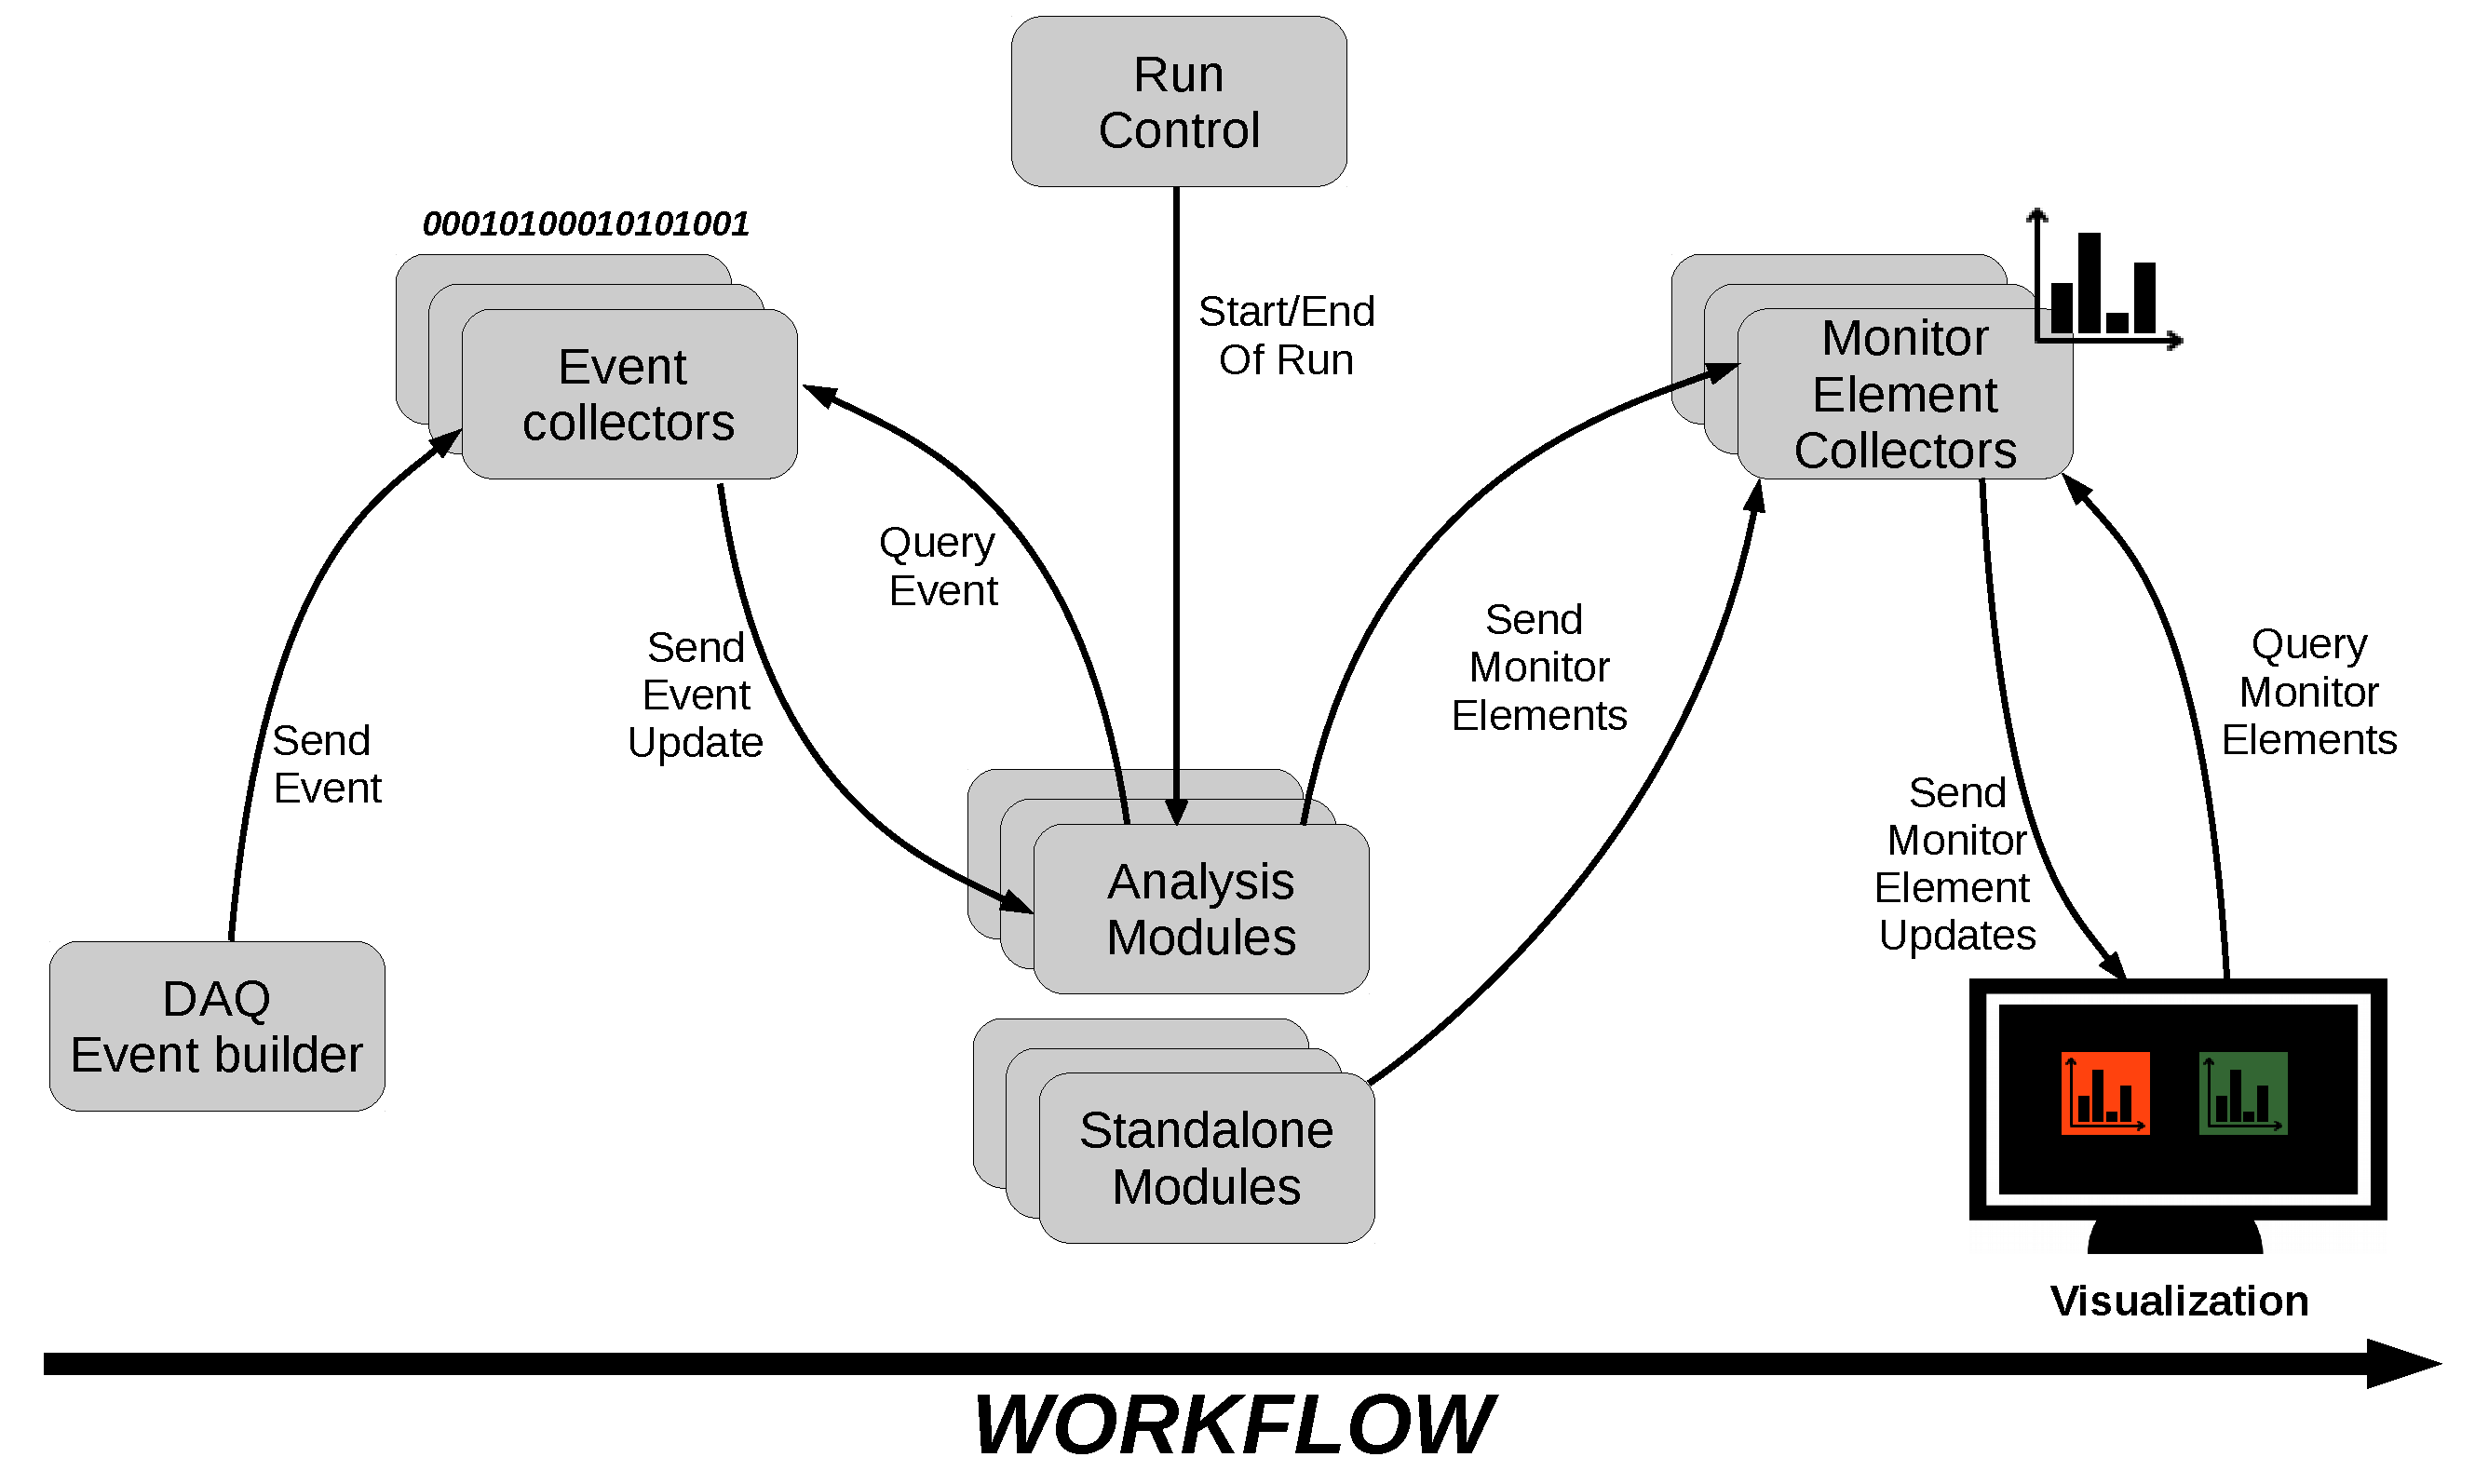
\includegraphics[width=\textwidth]{figs/DQM4HEP_workflow.pdf}        
    \end{center}
  
  \end{frame}
  
  %% EVENT COLLECTORS %%
  \begin{frame}[containsverbatim]
    \frametitle{\secname}
    \framesubtitle{Event collectors, client/server}
    
    \begin{minipage}{0.52\textwidth}
        Event collector (\verb|DQMEventCollector|) and \\
        Event client (\verb|DQMEventClient|) \\
        linked via DIM (TPC/IP).\\
        ~ \\
        Receiver interface with 2 modes :
        \begin{itemize}
          \item on update
          \item on query
        \end{itemize}
        ~ \\
        Sender interface with one unique command to send an event to the collector server \\
        ~ \\
        Use \verb|dqm4hep_start_event_collector| to start a collector server.
    \end{minipage}
    \begin{minipage}{0.42\textwidth}
      \begin{center}
        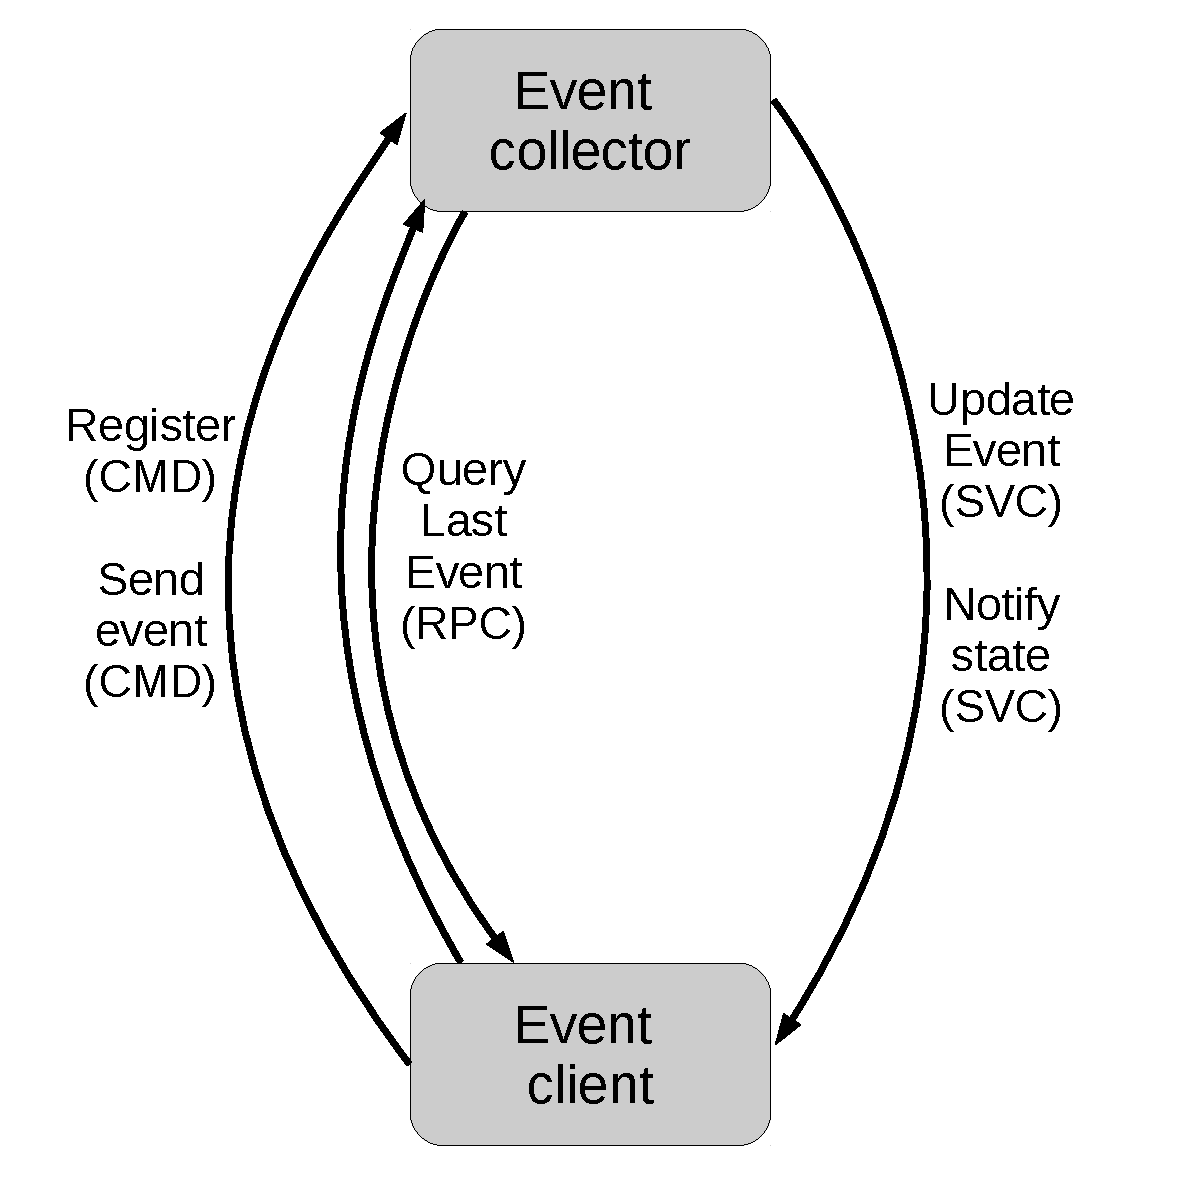
\includegraphics[width=\textwidth]{figs/event_collector_arch.pdf}        
      \end{center}      
    \end{minipage}
        
  \end{frame}

  
  %% MODULE APPLICATION %%
  \begin{frame}[containsverbatim]
    \frametitle{\secname}
    \framesubtitle{Module applications - analysis module}
    
    \begin{minipage}{0.78\textwidth}
      \begin{block}{Purpose}
        \begin{itemize}
          \item Receive events from a collector server and process them
          \item Produce monitor elements (histograms, scalars, generic TObject)
          \item Follow the run control signals (SOR, EOR)
        \end{itemize}
      \end{block}
              
      \begin{itemize}
        \item \textbf{Init} : Initialize the application : load dlls, declare services, etc ... Wait for a SOR
        \item \textbf{Start of run} : start cycles loop, open archive
        \item \textbf{Start of cycle} : start a cycle of '\textit{process event}'
        \item \textbf{Process event} : Process incoming event, fill monitor elements, etc ...
        \item \textbf{End of cycle} : send subscribed monitor elements, update archive (opt). 
        \item \textbf{End of run} : Wait for SOR, close archive (opt).
        \item \textbf{End} : Clean and exit module.
      \end{itemize}
      To implement online DQM analysis, user must implement the \verb|DQMAnalysisModule| interface. A shared library must be build and loaded in the application using the plugin system (see next slides). \\
      ~ \\
      Use \verb|dqm4hep_start_analysis_module| to start an analysis module.
        
    \end{minipage}
    \begin{minipage}{0.2\textwidth}
      \begin{flushright}
        \begin{tikzpicture}[scale=0.8]
        \node[draw] (I) at (0,-1) {Init};
        \node[draw] (SR) at (0,-2) {Start of run};
        \node[draw] (SC) at (0,-3) {Start of cycle};
        \node[draw] (PE) at (0,-4) {Process event};
        \node[draw] (EC) at (0,-5) {End of cycle};
        \node[draw] (ER) at (0,-6) {End of run};
        \node[draw] (E) at (0,-7) {End};
        \tikzset{fleche/.style={->,>=latex,thick}}
        \draw[fleche] (0,0) node {$\bullet$} -- (I);
        \draw[fleche] (I) -- (SR);
        \draw[fleche] (SR) -- (SC);
        \draw[fleche] (SC) -- (PE);
        \draw[fleche] (PE) -- (EC);
        \draw[fleche] (EC) -- (ER);
        \draw[fleche] (ER) -- (E);
        \draw[fleche] (E) -- (0,-8) node {$\bullet$};
        \draw[fleche] (0,-4.5) -- (1.3,-4.5) -- (1.3,-3.5) -- (0,-3.5);
        \draw[fleche] (0,-5.5) -- (1.4,-5.5) -- (1.4,-2.5) -- (0,-2.5);
        \draw[fleche] (0,-6.5) -- (1.5,-6.5) -- (1.5,-1.5) -- (0,-1.5);
        \end{tikzpicture}\\
        Analysis module~~~~\\ application flow~~~~~      
      \end{flushright}
    \end{minipage}
    
  \end{frame}
  
  \begin{frame}
    \frametitle{\secname}
    \framesubtitle{Module API}
      \begin{center}
       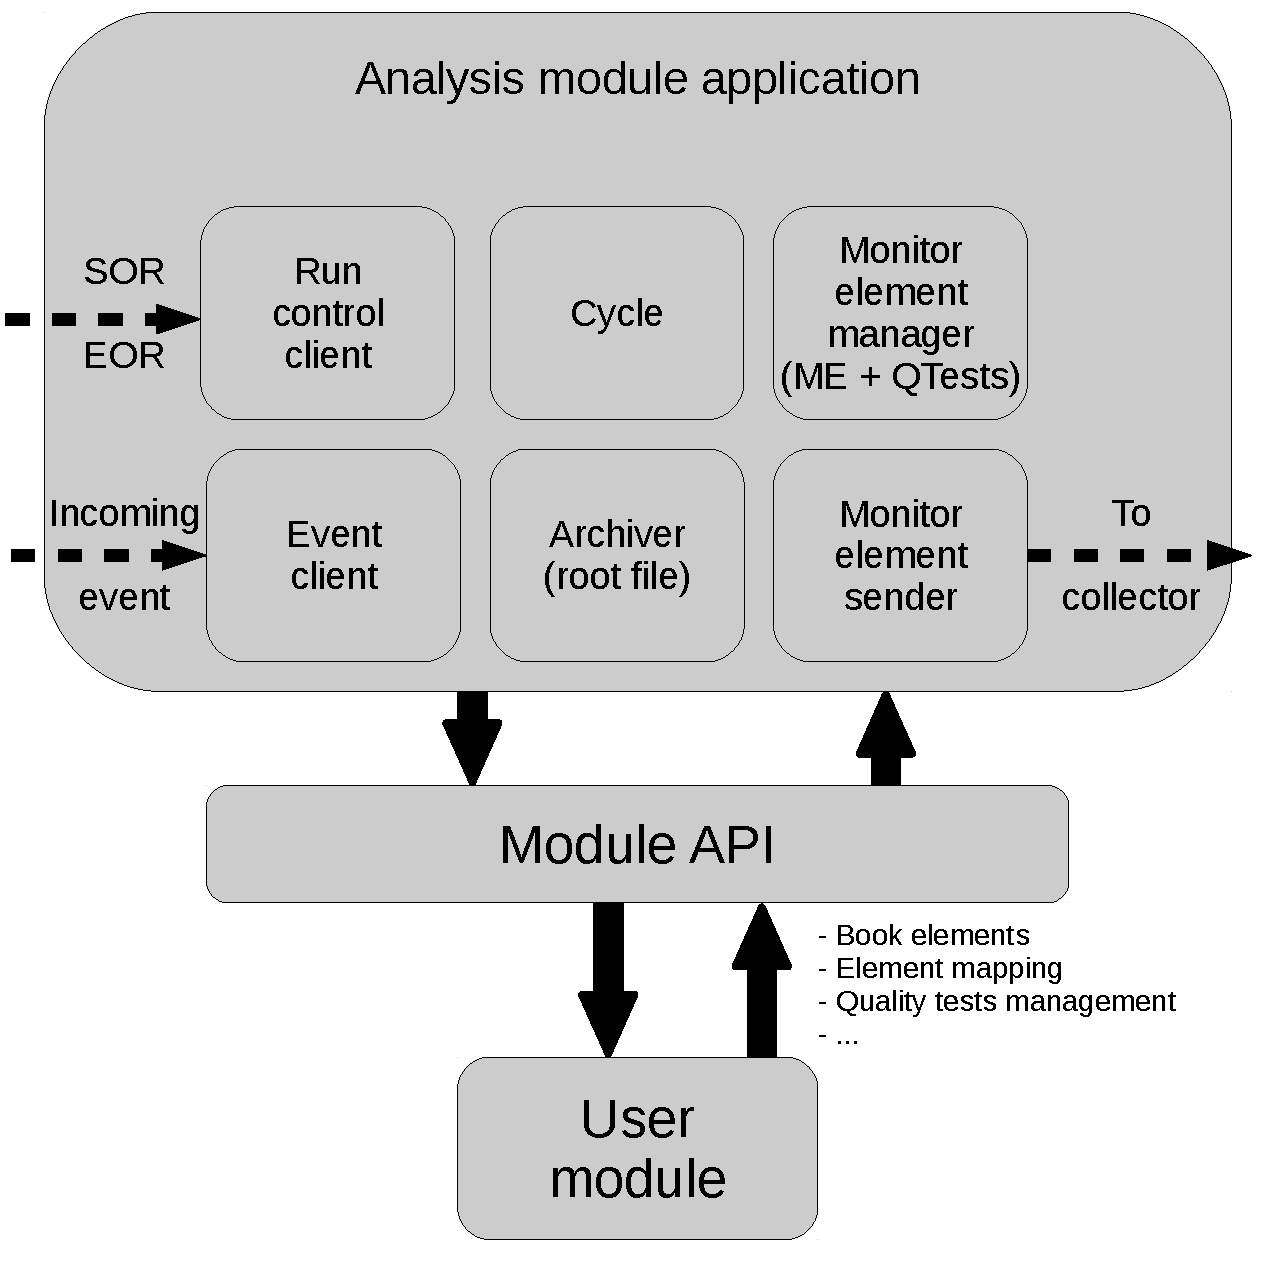
\includegraphics[width=0.6\textwidth]{figs/analysis_module_api.pdf}        
      \end{center}
  \end{frame}
  
  
  \begin{frame}[containsverbatim]
    \frametitle{\secname}
    \framesubtitle{Module applications - standalone module}
    
    \begin{minipage}{0.78\textwidth}
      \begin{block}{Purpose}
        \begin{itemize}
          \item No event reception
          \item No run signals
          \item Produce monitor elements (histograms, scalars, generic TObject)
        \end{itemize}
      \end{block}
      
      \begin{itemize}
        \item \textbf{Init} : Load dlls, init the module.
        \item \textbf{Start of cycle} : start a timer cycle of n seconds
        \item \textbf{Process} : call back function.
        \item \textbf{End of cycle} : collect monitor elements and send
        \item \textbf{End} : The application has received a signal to exit and the process ends.
      \end{itemize}
      To implement online standalone analysis, user must implement the \verb|DQMStandaloneModule| interface. A shared library must be build and loaded in the application using the plugin system (see next slides). \\
      ~ \\
      \textcolor{red}{Designed for \textit{slow control - like} data processing}. \\
      ~ \\
      Use \verb|dqm4hep_start_standalone_module| to start a standalone module.
    \end{minipage}
    \begin{minipage}{0.2\textwidth}
      \begin{flushright}
        \begin{tikzpicture}[scale=0.8]
        \node[draw] (I) at (0,-1) {Init};
        \node[draw] (SC) at (0,-2) {Start of cycle};
        \node[draw] (PE) at (0,-3) {Process};
        \node[draw] (EC) at (0,-4) {End of cycle};
        \node[draw] (E) at (0,-5) {End};
        \tikzset{fleche/.style={->,>=latex,thick}}
        \draw[fleche] (0,0) node {$\bullet$} -- (I);
        \draw[fleche] (I) -- (SC);
        \draw[fleche] (SC) -- (PE);
        \draw[fleche] (PE) -- (EC);
        \draw[fleche] (EC) -- (E);
        \draw[fleche] (E) -- (0,-6) node {$\bullet$};
        \draw[fleche] (0,-3.5) -- (1.3,-3.5) -- (1.3,-2.5) -- (0,-2.5);
        \draw[fleche] (0,-4.5) -- (1.4,-4.5) -- (1.4,-1.5) -- (0,-1.5);
        \end{tikzpicture} \\
        Standalone module~~~~\\ application flow~~~~~~~
      \end{flushright}
    \end{minipage}
    
  \end{frame}
  
  \begin{frame}
    \frametitle{\secname}
    \framesubtitle{Module API}
      \begin{center}
        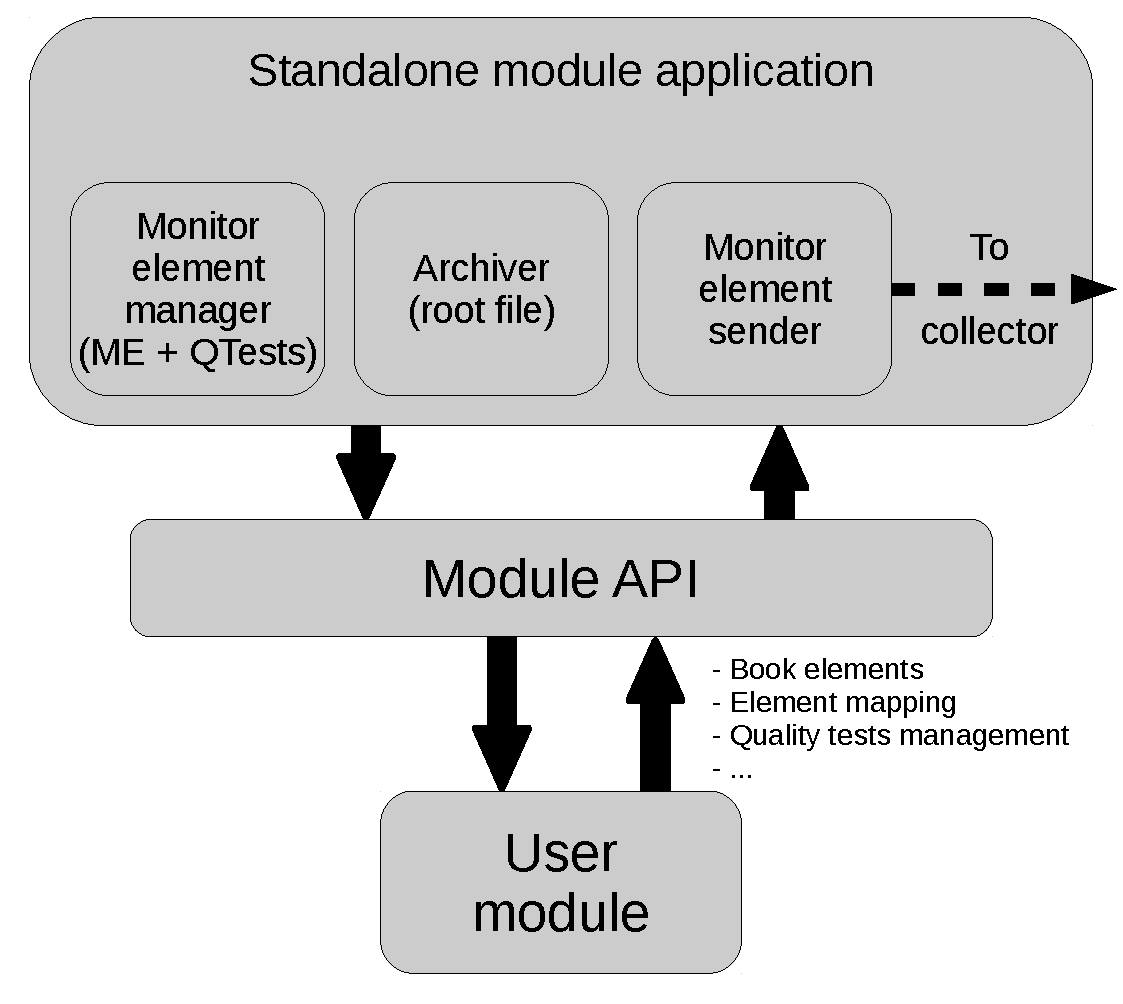
\includegraphics[width=0.6\textwidth]{figs/stand_module_api.pdf}        
      \end{center}
  \end{frame}
  
  %% MONITOR ELEMENT COLLECTOR %%

  \begin{frame}[containsverbatim]
    \frametitle{\secname}
    \framesubtitle{Monitor element collector, client/server}
    
    \begin{minipage}{0.43\textwidth}
      Collect monitor elements from different modules. \\
      ~ \\
      Publish/subscribe paradigm with client side. \\
      ~ \\
      Collector stores the available list of elements (names) from the different modules and the elements that the clients have subscribed.
    \end{minipage}
    \begin{minipage}{0.55\textwidth}
      \begin{center}
        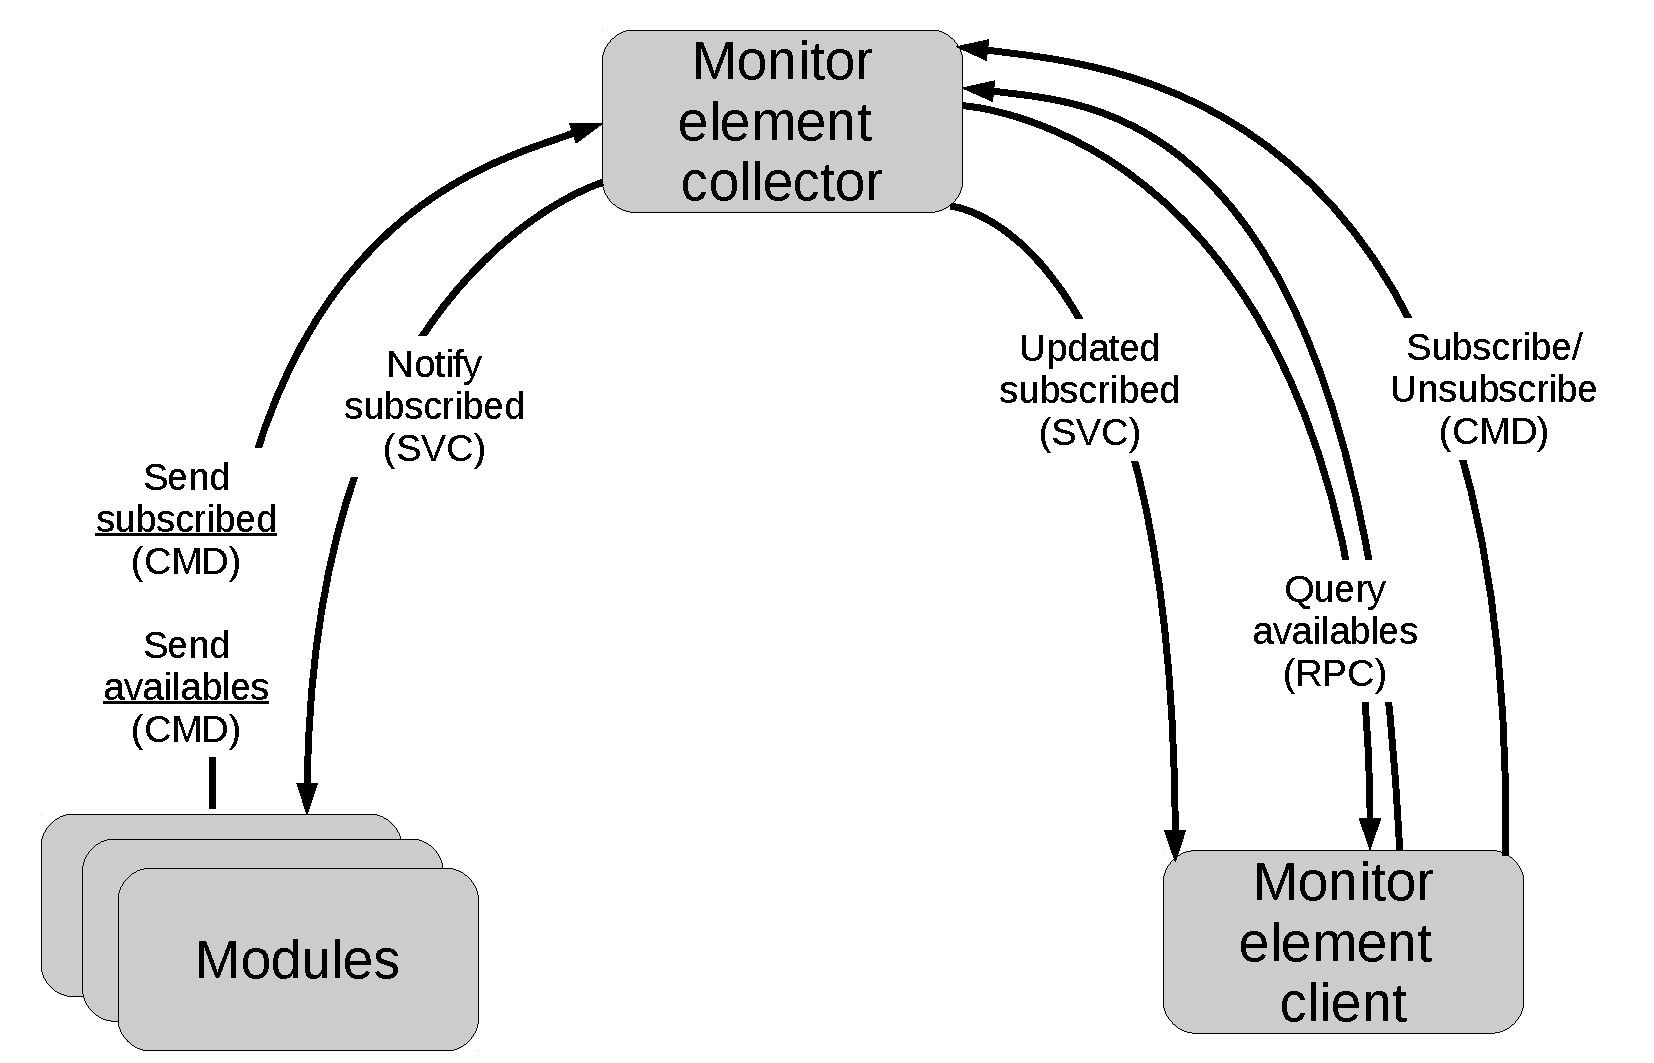
\includegraphics[width=\textwidth]{figs/me_collector_arch.pdf}        
      \end{center}      
    \end{minipage}
    ~ 
    ~ \\
    Client interface works on both update and query modes. \\
    ~ \\
    Use \verb|dqm4hep_start_monitor_element_collector| monitor element collector.
     
  \end{frame}
  



    %% USER INTERFACE OVERVIEW %%
    \section{User interfaces overview}
    
    \begin{frame}[containsverbatim]
      \frametitle{\secname}
      \framesubtitle{Plugin system}
      
      The core part of the system provides a plugin system, massively used by the framework to handle user classes. \\
      ~ \\
      The \verb|DQMPluginManager| singleton class manages the plug-ins provided by the system and the users. Plugins can be loaded at any time by loading shared libraries. \\
      ~ \\
      Example :
      \begin{lstlisting}
      // single library loading
      DQMPluginManager::instance()->loadLibrary("libMyClass.so"); 
      // multiple libraries loading
      StringVector libraries = { "libMyClass.so" , "libAnotherClass.so" }
      DQMPluginManager::instance()->loadLibraries(libraries); 
      // using DQM4HEP_PLUGIN_DLL env var with ':' separation
      // assuming export DQM4HEP_PLUGIN_DLL=./lib/libSuperClass.so:./lib/libDirtyClass.so
      DQMPluginManager::instance()->loadLibraries(); 
      \end{lstlisting}
      
      ~ \\
      In principle \textbf{any} user class can be plugged in the framework and retrieved inside applications. \\
      ~ \\
    \end{frame}
    
    
    \begin{frame}[containsverbatim]
      \frametitle{\secname}
      \framesubtitle{Plugin system}
      User Example :
      \begin{lstlisting}
      // MyClass.h
      class MyClass 
      {
        public:
          MyClass(); // Default constructor mandatory !!
        private:
          int    m_attribute;
      };
      // MyClass.cc
      DQM_PLUGIN_DECL( MyClass , "MyClass" ) // plug the class in the system
      
      MyClass::MyClass() : m_attribute(0) {}
      // ...
      \end{lstlisting}
      %\pause

      To get an instance of your class, use the plugin manager :
      \begin{lstlisting}
      // ...
      MyClass *pClass = DQMPluginManager::instance()->createPluginClass<MyClass>("MyClass");
      // ...
      \end{lstlisting}
      
      For example, this functionality is used internally to get :
      \begin{itemize}
        \item user module implementations
        \item event streamers
        \item run control clients
      \end{itemize}

    \end{frame}
    
    
    
    
    %% STREAMER INTERFACE %%
    \begin{frame}[containsverbatim]
    \frametitle{\secname}
    \framesubtitle{Streaming interface}

      \textbf{The framework has \textcolor{red}{no dependency on the type of data} transferred over the network!} \\
      ~ \\
      For example, the streamer for LCIO is implemented and provided as a plug-in in the software. The type of data that is transferred over the network can be user defined. \\
      Users have to implements the \verb|DQMEventStreamer| interface : \\

  \begin{lstlisting}
  class DQMEventStreamer : public DQMStreamer<DQMEvent>
  {
  public:
    // ...
    virtual StatusCode serialize(const DQMEvent *const pEvent, DQMDataStream *const pDataStream) = 0;
    virtual StatusCode deserialize(DQMEvent *&pEvent, DQMDataStream *const pDataStream) = 0;
    virtual StatusCode serialize(const DQMEvent *const pEvent, const std::string &subEventIdentifier, DQMDataStream *const pDataStream) = 0;
  };
  \end{lstlisting}
  
  and plug the streamer class using the plugin mechanism. The \verb|DQMDataStream| class provides functions to read and write raw buffers. \\
  ~ \\
  For an experiment with a simple event structure, it can be useful to define a raw event streamer and propagate the event through the DQM system without taking care about the network interface. \\
    \end{frame}
  
  
  \begin{frame}
    \frametitle{\secname}
    \framesubtitle{Gui visualisation}
        
	  Gui interfaces for DQM client developed :
            
      \begin{itemize}
        \item Run control, job control, online monitoring
        \item Written with Qt4 framework     
\includegraphics[width=.03\textwidth]{logo/Qt_CMYK_color}
        \item Easily configurable with json and xml.
      \end{itemize}
    
      \end{frame} 
      
      
 %% Run Control %%
 \begin{frame}
    \frametitle{\secname}
    \framesubtitle{ Run Control GUI }
    \begin{center}
      \begin{overlayarea}{\textwidth}{\textheight}
        \begin{center}
          \begin{onlyenv}<1>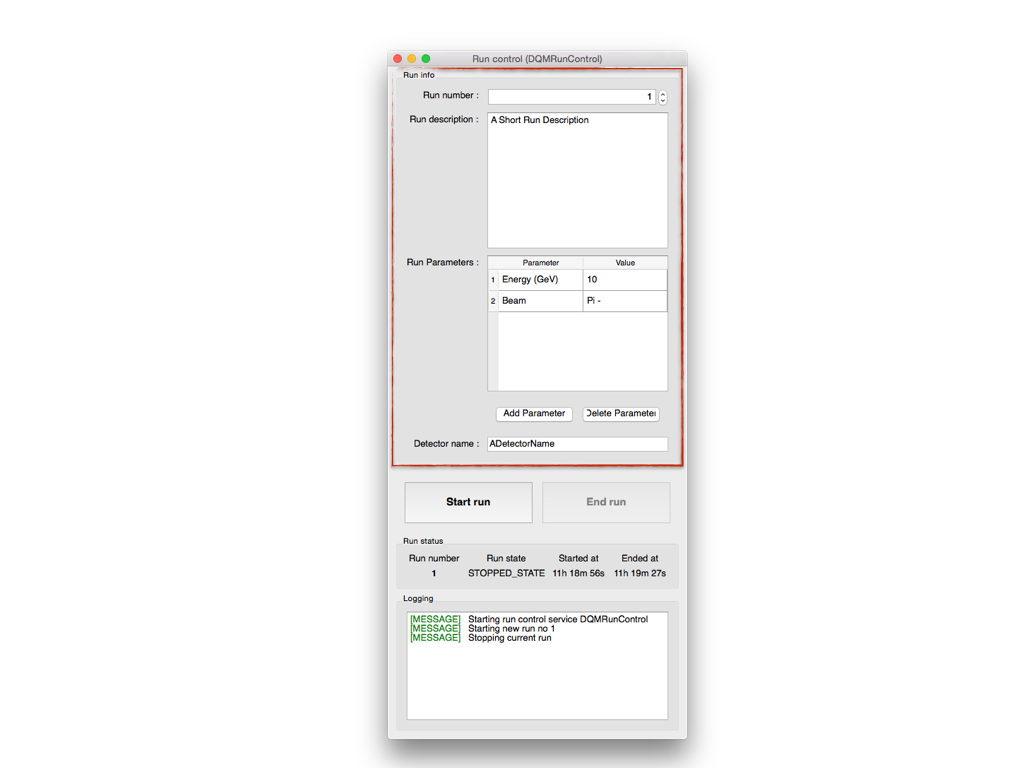
\includegraphics[width=0.8\textwidth]{figs/RunControl/RunControl_Infos.png}\end{onlyenv}
          \begin{onlyenv}<2>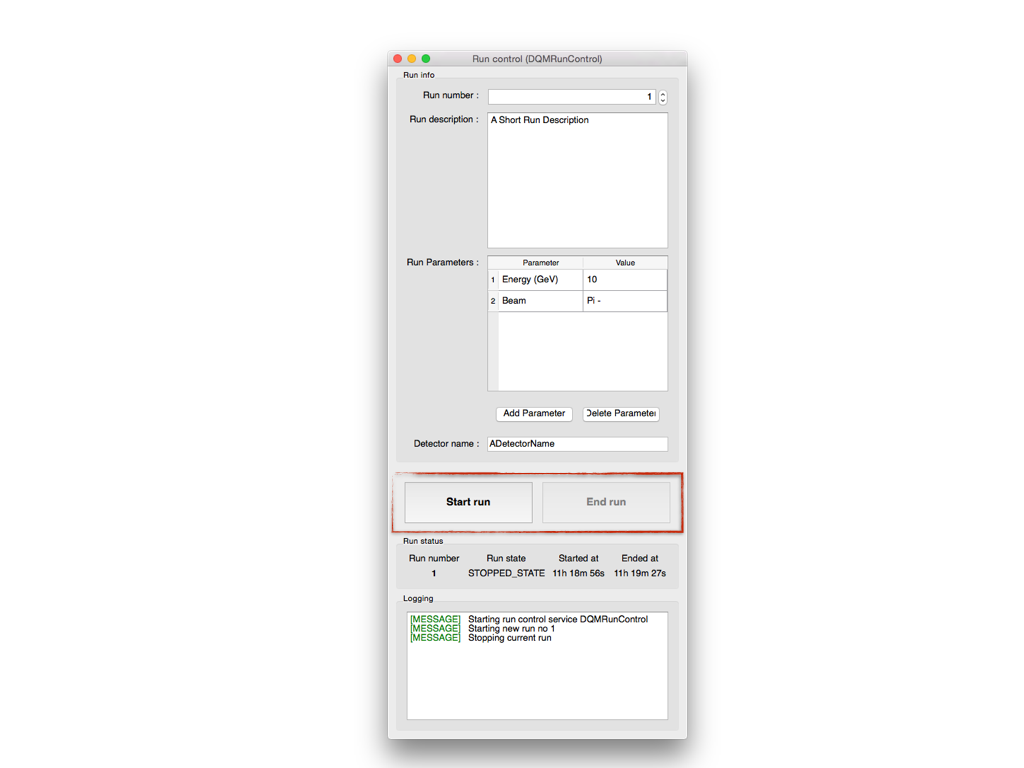
\includegraphics[width=0.8\textwidth]{figs/RunControl/RunControl_SOR.png}\end{onlyenv}
          \begin{onlyenv}<3>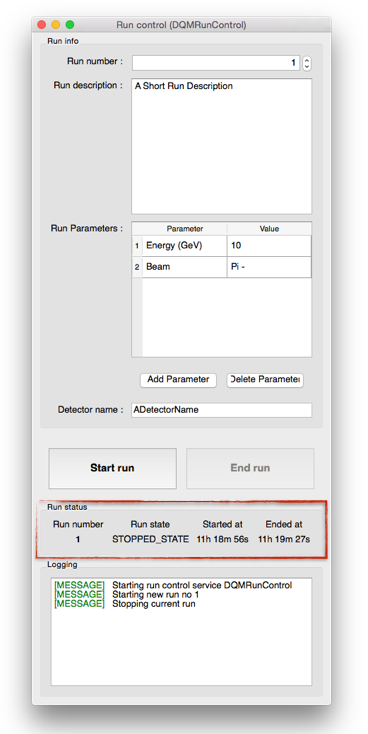
\includegraphics[width=0.8\textwidth]{figs/RunControl/RunControl_Status.png}\end{onlyenv}
          \begin{onlyenv}<4>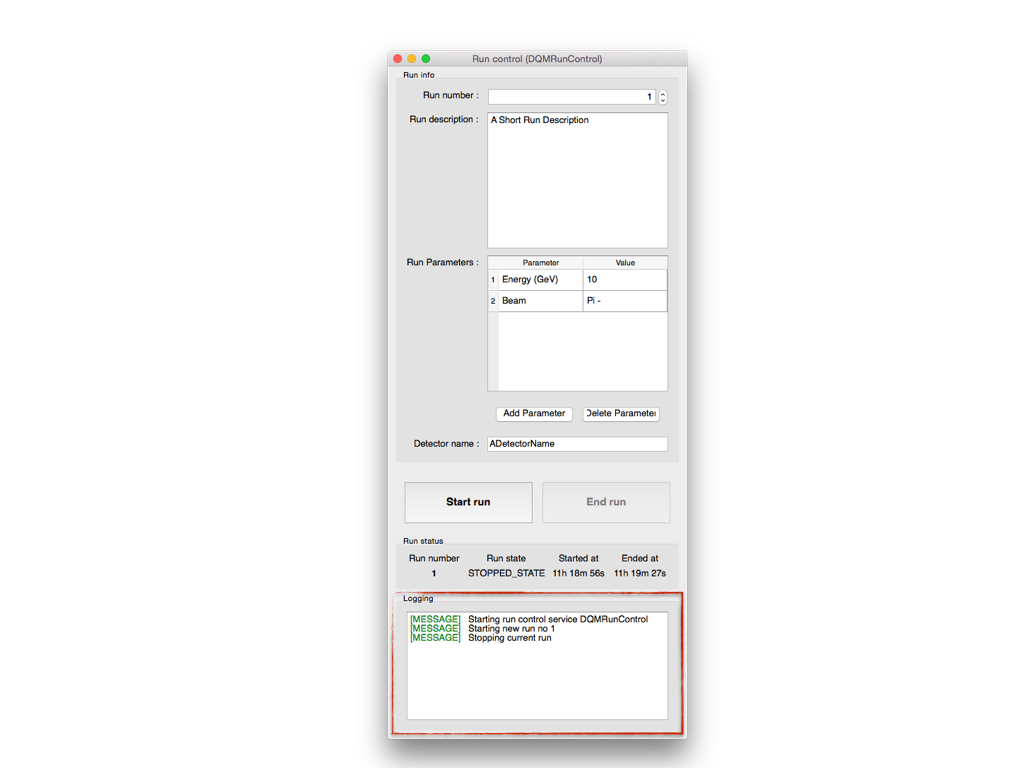
\includegraphics[width=0.8\textwidth]{figs/RunControl/RunControl_logging.png}\end{onlyenv}
        \end{center}
      \end{overlayarea}
    \end{center}
  \end{frame}
   
       
 %% Job Interface %%
  \begin{frame}
    \frametitle{\secname}
    \framesubtitle{ Job Control GUI }
      \begin{overlayarea}{\textwidth}{\textheight}
      \begin{center}
        \begin{onlyenv}<4>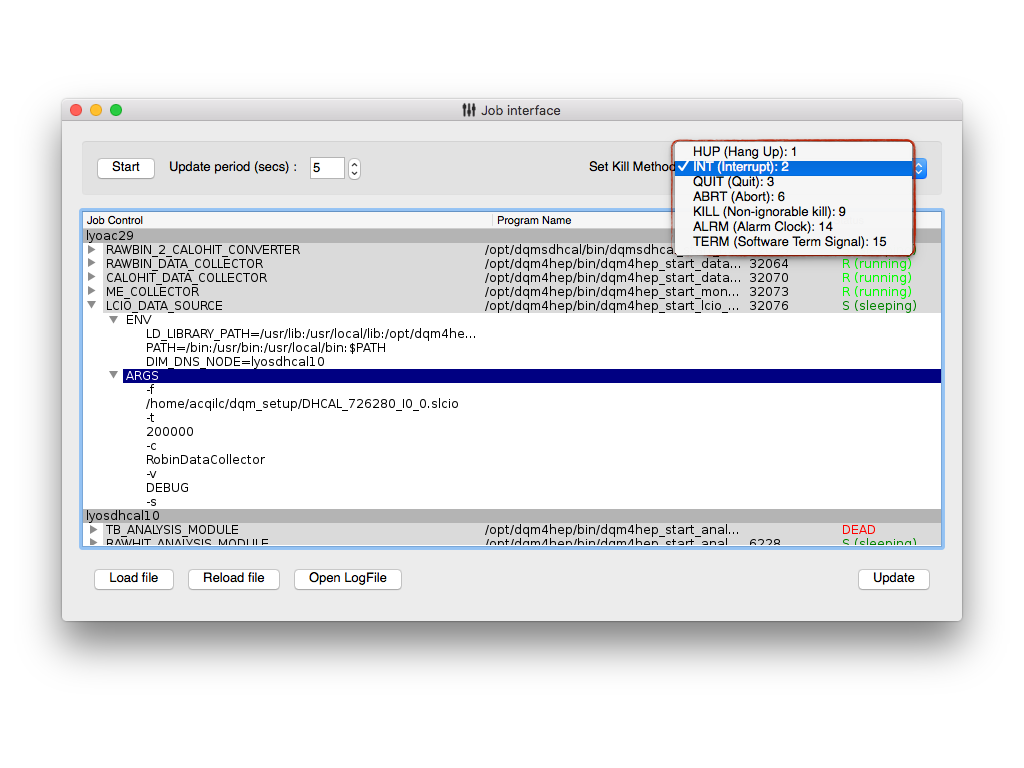
\includegraphics[width=0.8\textwidth]{figs/JobInterface/JobInterface_KillSwitch.png}\end{onlyenv}
        \begin{onlyenv}<2>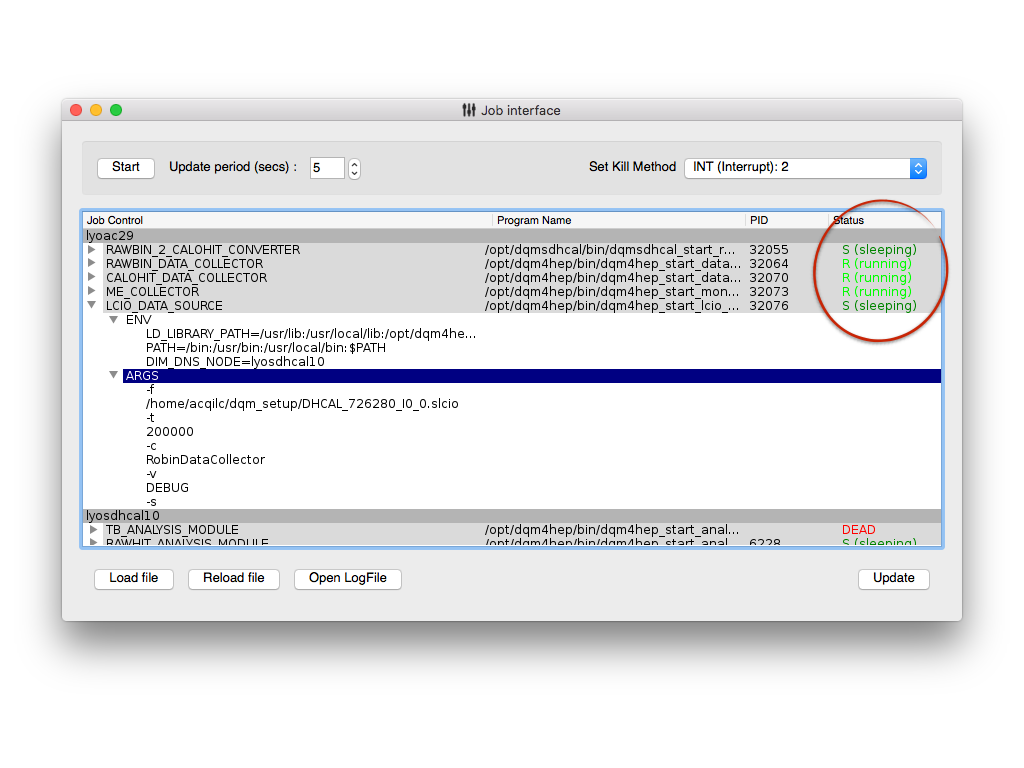
\includegraphics[width=0.8\textwidth]{figs/JobInterface/JobInterface_LiveStatus.png}\end{onlyenv}
        \begin{onlyenv}<3>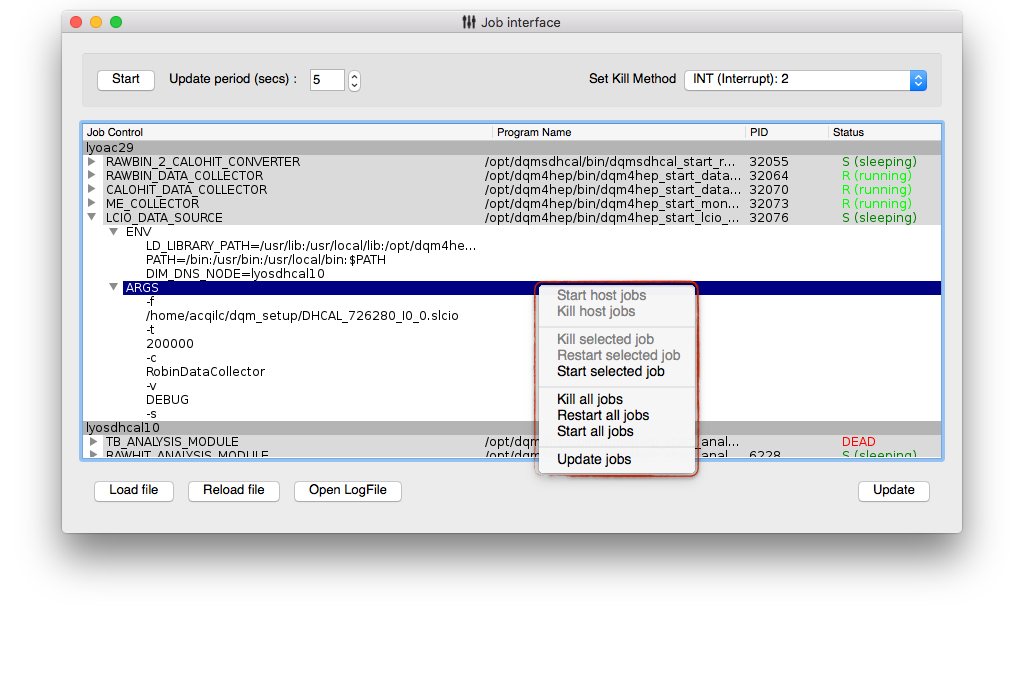
\includegraphics[width=0.8\textwidth]{figs/JobInterface/JobInterface_Module.png}\end{onlyenv}
        \begin{onlyenv}<1>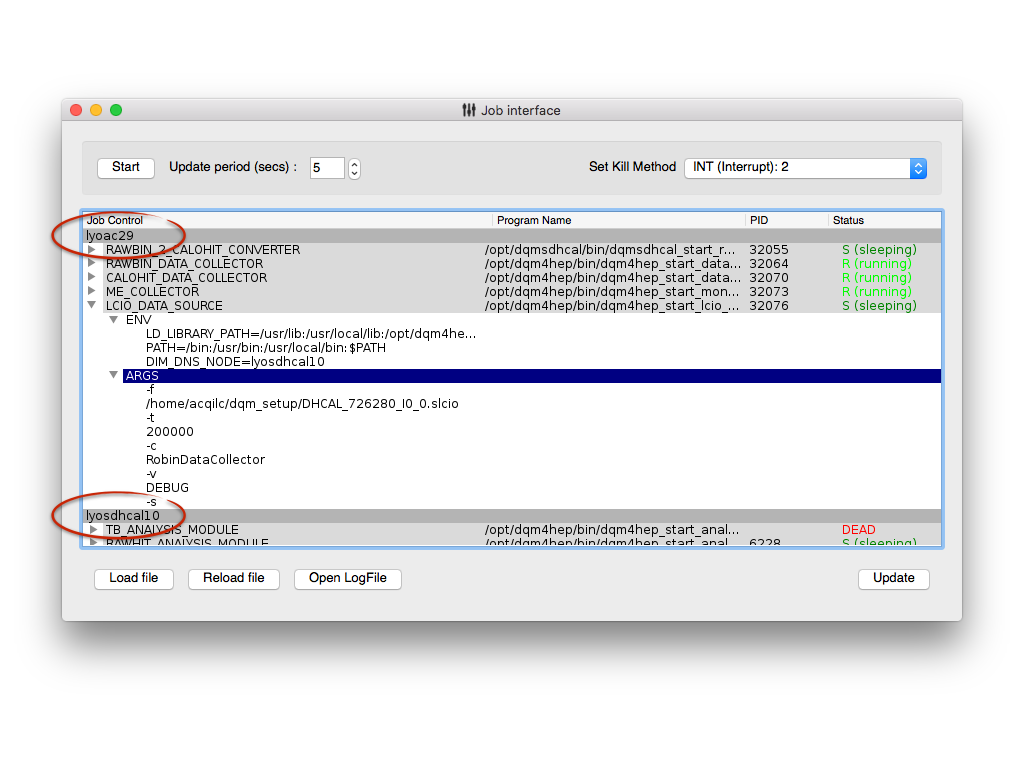
\includegraphics[width=0.8\textwidth]{figs/JobInterface/JobInterface_MultiHost.png}\end{onlyenv}
        \begin{onlyenv}<5>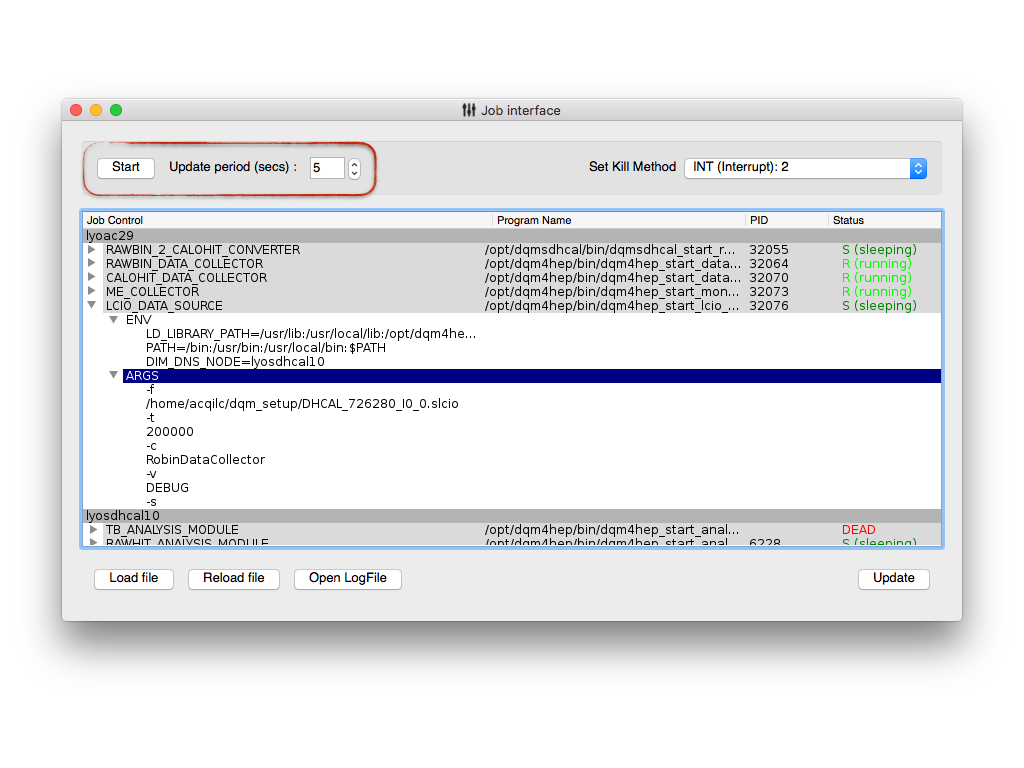
\includegraphics[width=0.8\textwidth]{figs/JobInterface/JobInterface_Update.png}\end{onlyenv}
      \end{center}
    \end{overlayarea}
  \end{frame}
  
  
   %% Monitoring Control %%
 \begin{frame}
    \frametitle{\secname}
    \framesubtitle{ Monitoring Gui }
    
    \begin{overlayarea}{\textwidth}{\textheight}
      \begin{center}
        \begin{onlyenv}<1>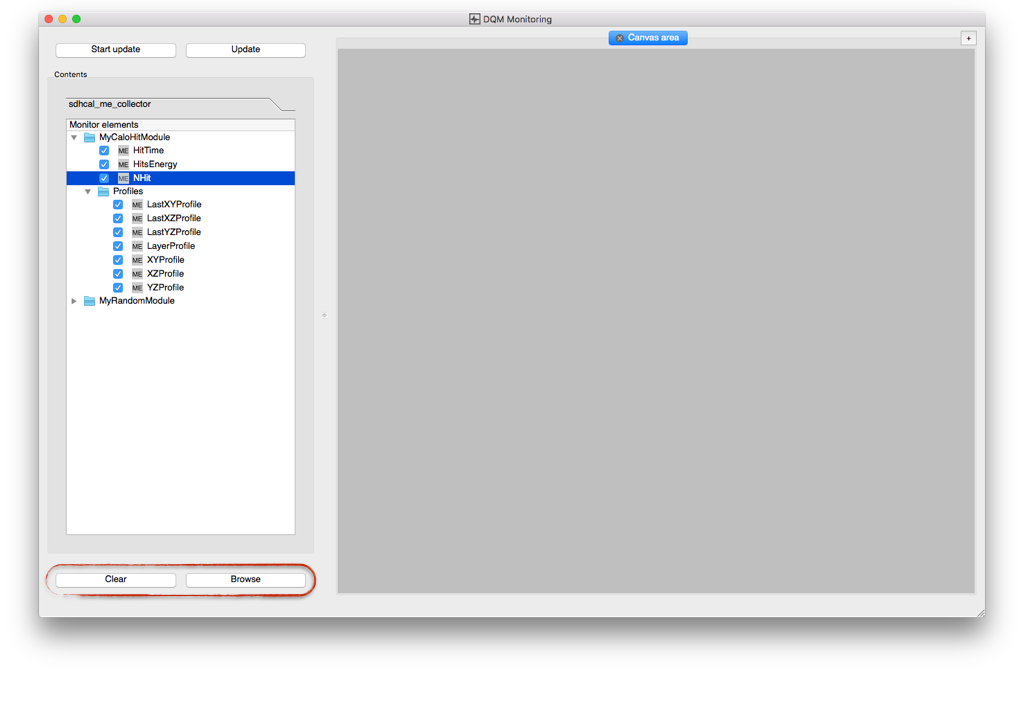
\includegraphics[width=0.8\textwidth]{figs/MonitoringGui/MG_Browse.png}\end{onlyenv}
        \begin{onlyenv}<2>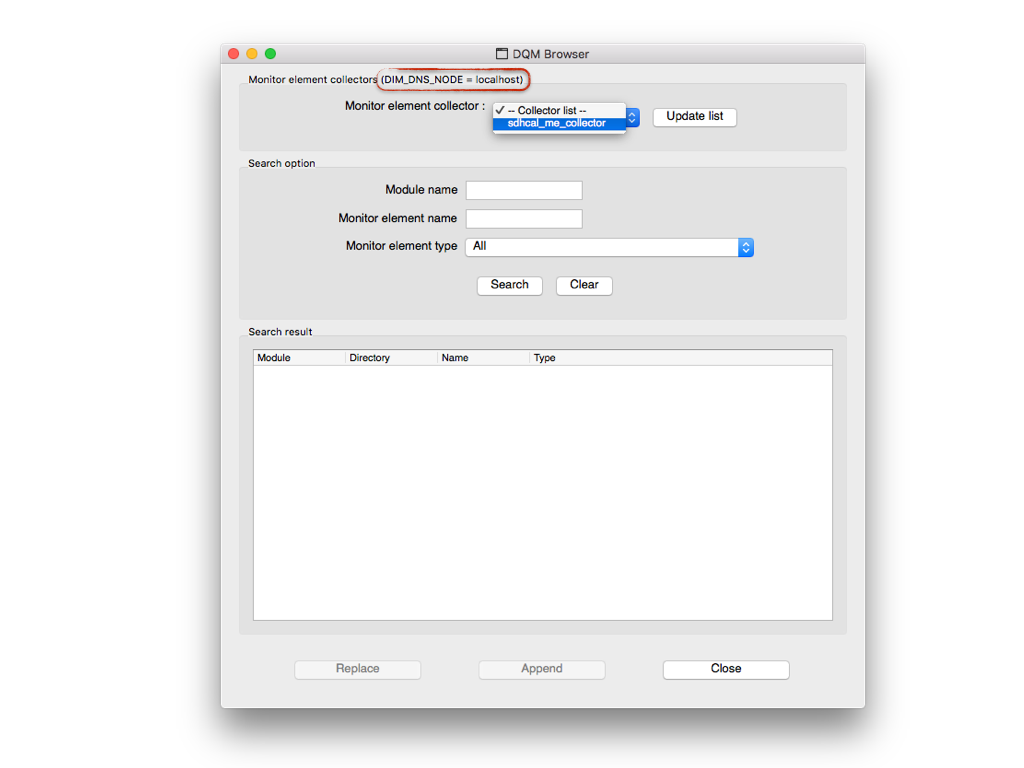
\includegraphics[width=0.8\textwidth]{figs/Browser/Browser_DNSNode.png}\end{onlyenv}
%         \begin{onlyenv}<3>\includegraphics[width=0.8\textwidth]{figs/MonitoringGui/}\end{onlyenv}
%         \begin{onlyenv}<4>\includegraphics[width=0.8\textwidth]{figs/MonitoringGui/}\end{onlyenv}
%         \begin{onlyenv}<5>\includegraphics[width=0.8\textwidth]{figs/MonitoringGui/}\end{onlyenv}
%         \begin{onlyenv}<6>\includegraphics[width=0.8\textwidth]{figs/MonitoringGui/}\end{onlyenv}
%         \begin{onlyenv}<7>\includegraphics[width=0.8\textwidth]{figs/MonitoringGui/}\end{onlyenv}
%         \begin{onlyenv}<8>\includegraphics[width=0.8\textwidth]{figs/MonitoringGui/}\end{onlyenv}
%         \begin{onlyenv}<9>\includegraphics[width=0.8\textwidth]{figs/MonitoringGui/}\end{onlyenv}
%         \begin{onlyenv}<10>\includegraphics[width=0.8\textwidth]{figs/MonitoringGui/}\end{onlyenv}
%         \begin{onlyenv}<11>\includegraphics[width=0.8\textwidth]{figs/MonitoringGui/}\end{onlyenv}
%         \begin{onlyenv}<12>\includegraphics[width=0.8\textwidth]{figs/MonitoringGui/}\end{onlyenv}
%         \begin{onlyenv}<13>\includegraphics[width=0.8\textwidth]{figs/MonitoringGui/}\end{onlyenv}
%         \begin{onlyenv}<14>\includegraphics[width=0.8\textwidth]{figs/MonitoringGui/}\end{onlyenv}
%         \begin{onlyenv}<15>\includegraphics[width=0.8\textwidth]{figs/MonitoringGui/}\end{onlyenv}
      \end{center}
    \end{overlayarea}
    
  \end{frame}
    
    
    
  %%%%%%%%%%%
  %% TESTS %%
  %%%%%%%%%%%  
  
  \section{DQM4HEP tests}

  \begin{frame}
  \frametitle{\secname}

  Tests of the framework were performed using the SDHCAL electronics (SDHCAL Difs). \\
  Ideas were to test : \\
  
  \begin{itemize}
    \item Easy to deploy ? configure ?
    \item Easy to use interfaces ?
    \item Network saturation with many analysis
    \item Test specific SDHCAL DQM tools :
    \begin{itemize}
      \item Raw data converter service (Streamout)
      \item Event reconstruction tool (Trivent)
      \item Online analysis
      \item Online data taking (/dev/shm reader)
    \end{itemize}
  \end{itemize}
  
  \end{frame}
  
  
  \begin{frame}
  \frametitle{\secname}
  \framesubtitle{Deployment}
  
  \centering 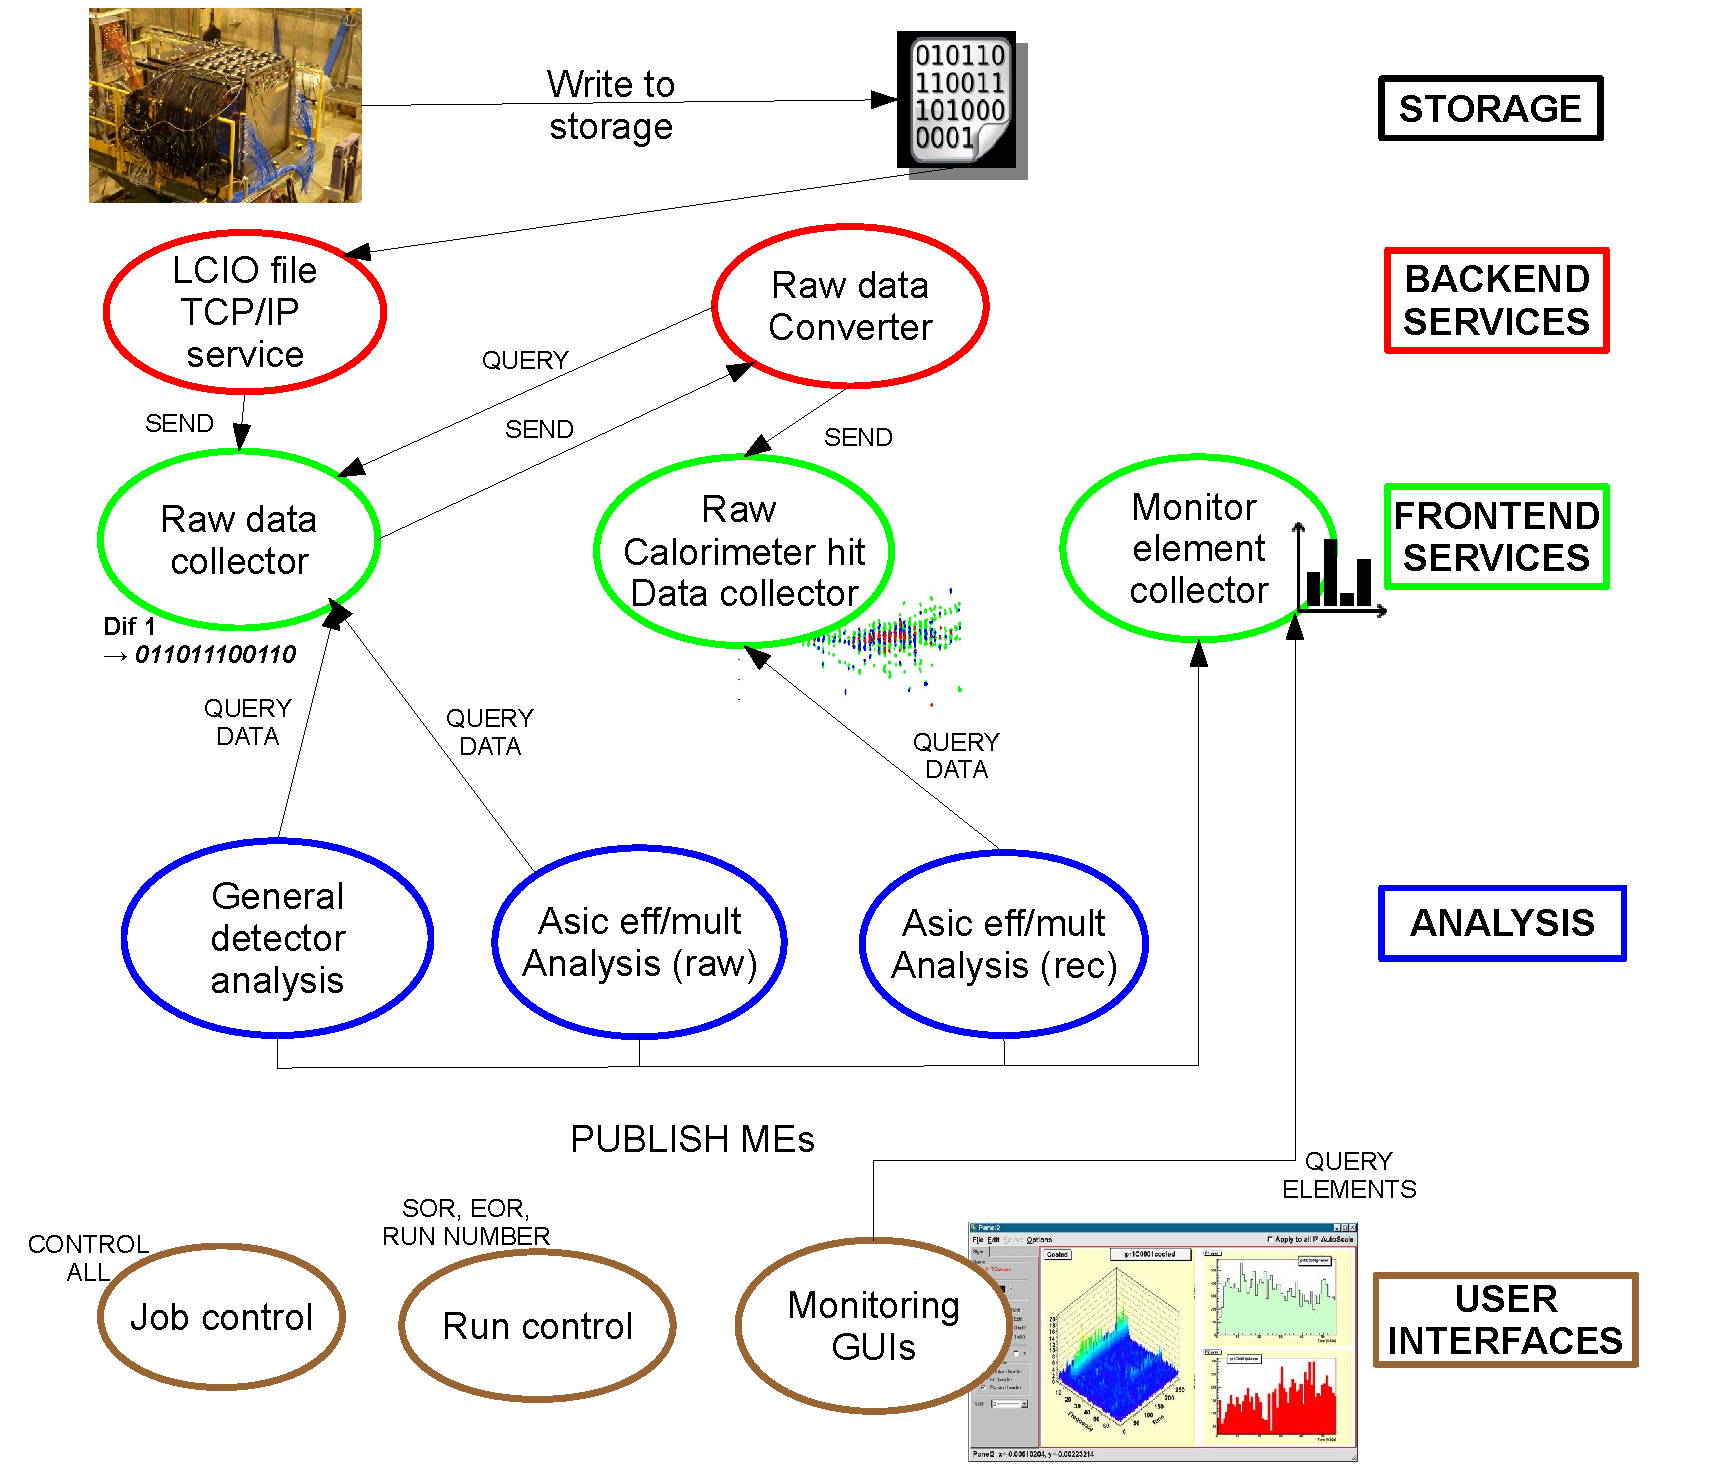
\includegraphics[width=0.72\textwidth]{figs/DQM4HEP_DEPLOYEMENT_TEST.pdf}
  
  \end{frame}
  
  
  \begin{frame}
  \frametitle{\secname}
  \framesubtitle{Results}

  \textbullet ~~ Easy package installation/update (CMake + GIT) \\
  ~ \\
  
  \textbullet ~~ Input file : SDHCAL TB December 726280 (20 GeV pion run) \\
  ~ \\  

  \textbullet ~~ Job control really makes life easier ! \\
  Easy to start, stop, restart and reconfigure programs. Easy to detect configuration problems ! \\
  ~ \\
  \begin{minipage}{0.6\textwidth}
    Gui can display :
    \begin{itemize}
      \item total efficiency mapping (47 plots)
      \item total multiplicity mapping (47 plots)
      \item global efficiency/multiplicity and statistics (4 plots) 
    \end{itemize}

    at the same time, with frequent updates (every 5 seconds) without lagging. Gui handling still ok.
  \end{minipage}
  \begin{minipage}{0.38\textwidth}
    \begin{center}
      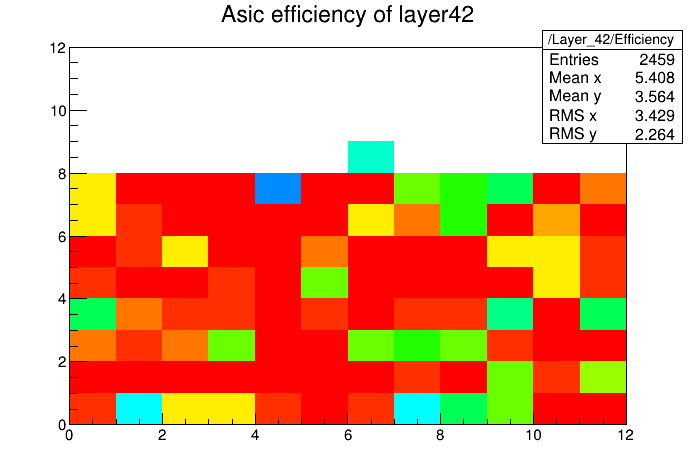
\includegraphics[width=\textwidth]{figs/AsicEff42.png} \\
      Disconnected DIF in layer 42 !
    \end{center}
  \end{minipage}
  
  More tests : \\
  ~ \\
  \textbullet ~~ Static code analyser (cppcheck) : no errors, POSIX norm ok \\
  ~ \\
  \textbullet ~~ Online data taking (/dev/shm) : OK ! \\
  ~ \\
  
  \end{frame}
  
  
  \begin{frame}
  \frametitle{\secname}
  \framesubtitle{Conclusions and plans}

  \begin{block}{Conclusion}
    \begin{itemize}
      \item Network decouples/links different part of the system.
      \item Plugins (modules, data streaming) to configure and run the system 
      \item Tools for data feed in the system from the DAQ (event client interface)
      \item GUIs to control/monitor the system
      \item Tests OK, numbers ... ?
    \end{itemize}
  \end{block}
  
  \begin{block}{Plans}
    \begin{itemize}
      \item Full implementation of SDHCAL DQM :
      \begin{itemize}
        \item Gas system, HV, LV, T/P
        \item Global detector (efficiency, multiplicity, nHit 1-2-3, rate)
        \item Particle ID (counting, selection)
        \item Particle specific modules (pion, electron, muons)
        \item Energy reconstruction
        \item Particle flow (performance)
      \end{itemize}
      \item Performance tests : timing, statistics, compression (network, streaming)
      \item Reimplementation of some interfaces (networking)
      \item ILCSOFT ?
      \item Combined ECAL test-beam : combined DQM ? 
    \end{itemize}
  \end{block}
  
  \end{frame}
  
  %%%%%%%%%%%%%%%%
  %% CONCLUSION %%
  %%%%%%%%%%%%%%%%
  
 
  \begin{frame}
  
  ~ \\
  ~ \\
  ~ \\
  ~ \\
  ~ \\
  ~ \\
    \centering \large Thanks for your attention
  ~ \\
  ~ \\
  ~ \\
  
    
  \end{frame}

\end{document}
